\todo{actual biological terms}

Consider an open and bounded set $U \subseteq \R^d$ with $C^1$ boundary and $T > 0$. This can be interpreted as the microscopic part of the body we are investigating. We identify the cells in this part of the body by an open set $C \subseteq U$, also with $C^1$ boundary, and the extracellular space by $\Omega := U \setminus \overline{C}$. We require that the closure $\overline{C}$ of $C$ is also completely contained in $U$, i.e. no cells should touch the boundary of our domain. In particular, this implies that the boundary $\partial \Omega$ of the extracellular space can be written as the disjoint union of the boundary of our region of investigation $\partial U$ and the cell membranes $\partial C$, which we denote by $\Gamma_{e}$ and $\Gamma$, respectively. We use the function $u: [0, T] \times \Gamma \to \R$ to represent the concentration of free receptors at a given time and location on a cell membrane. Similarly, $u_b: [0, T] \times \Gamma \to \R$ represents the concentration of bounded receptors, and $v: [0, T] \times \overline{\Omega} \to \R$ represents the concentration of ligands in $\overline{\Omega}$, see \cref{fig:domain}.

\begin{figure}[!t]
    \centering
    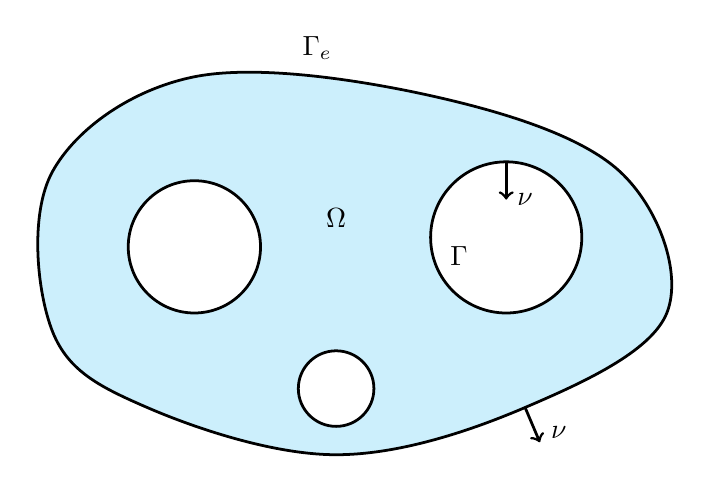
\begin{tikzpicture}[scale=1.2]

    \fill[cyan!20, even odd rule]
    plot[smooth cycle, tension=0.6] coordinates {
        (-3,1.5)
        (-1.5,2.5)
        (1,2.3)
        (3,1.5)
        (3.5,0)
        (2,-1)
        (0,-1.5)
        (-2,-1)
        (-3,-0.2)
    }
    (-1.5,0.7) circle (0.7)
    (1.8,0.8) circle (0.8)
    (0,-0.8) circle (0.4);
    
    % Outer irregular boundary
    \draw[line width=1pt]
      plot[smooth cycle, tension=0.6] coordinates {
        (-3,1.5)
        (-1.5,2.5)
        (1,2.3)
        (3,1.5)
        (3.5,0)
        (2,-1)
        (0,-1.5)
        (-2,-1)
        (-3,-0.2)
      };
    
    % Inner circles
    \draw[line width=1pt] (-1.5,0.7) circle (0.7);
    \draw[line width=1pt] (1.8,0.8) circle (0.8);
    \draw[line width=1pt] (0,-0.8) circle (0.4);
    
    % Labels
    \node at (0.0,1.0) {$\Omega$};
    \node at (1.3,0.6) {$\Gamma$};
    \node at (-0.2,2.8) {$\Gamma_e$};
    \node at (2.0,1.2) {$\nu$};
    \node at (2.356, -1.268) {$\nu$};
    
    % Arrows (boundary directions)
    \draw[->, line width=1pt] (1.8,1.6) -- (1.8,1.2);
    \draw[->, line width=1pt] (2,-1) -- (2.156, -1.368);
    
    \end{tikzpicture}
    \caption{A sketch of a possible domain in the case that $d= 2$. The blue background represents $\Omega$ and the two kinds of boundaries are indicated, along with the outward unit normal vector $\nu$.}
    \label{fig:domain}
\end{figure}

The ligands can move freely through the extracellular space. This can be modelled by the standard diffusion (or heat) equation. To simplify the setting\todo{setting?}, we assume the individual receptors will be fixed in their position on the cell membrane.

When a ligand binds to a free receptor, the concentration of free receptors and ligands decrease, and the concentration of bounded receptors at that position increases accordingly. This reaction is described by $\kon u^2 v$ for some $\kon > 0$. After some time, the bounded receptor has done its task, passing the signal through to the interior of the cell. It releases the ligand and is now available to bind to a new ligand again. The concentration of bounded receptors decrease, and the concentration of free receptors and ligands increase accordingly. The rate of this dissociation is described by $\koff u_b$, where $\koff > 0$.

Finally, two reactions that happen constantly are production and decay. To keep intercellular communication possible, cells produce ligands and receptors that enter the domain $\Omega$ through the cell membrane. We assume the production of ligands and free receptors mainly happens at constant rates $P_u > 0$ and $P_v > 0$, but is also upregulated by the concentration of bounded receptors, which is taken into account by $\alpha u_b$ for some upregulation coefficient $\alpha > 0$. The ligands, free receptors and complex receptors decay at constant rates $\delta_v$, $\delta_u$ and $\delta_{u_b}$, respectively.

We can describe the dynamics of ligands and receptors by a system of coupled differential equations. Denote the diffusion coefficient by $D_v > 0$ and the outward unit normal vector on $\partial \Omega$ by $\nu$. Then the concentrations of receptors can then be described by the system of ODEs given by

\begin{equation}
    \label{sys:ODEs}
    \begin{aligned}
        u_t         &= P_u + \alpha u_b - \delta_u u - 2 \kon u^2 v + 2 \koff u_b   & \text{on }& (0, T) \times \Gamma, \\
        u_{b,t}     &= -\delta_{u_b} u_b + \kon u^2 v - \koff u_b                   & \text{on }& (0, T) \times \Gamma. \\
    \end{aligned}
\end{equation}

\noindent
Note that even though they are given by only two equations, this is actually a system of uncountably many ODEs. For every boundary point $x \in \Gamma$, we have one ODE for the function $t \mapsto u(t, x)$ and one for the function $t \mapsto u_b(t, x)$.

Since the dynamics of the ligands include diffusion in $\Omega$ and reaction on $\Gamma$, they can be described by the PDE and boundary conditions given by

\begin{equation}
    \label{sys:PDEs}
    \begin{aligned}
        v_t                   &= D_v \Delta v - \delta_v v      & \text{in }& (0, T) \times \Omega, \\
        D_v \pderiv[v]{\nu}   &= P_v - \kon u^2 v + \koff u_b   & \text{on }& [0, T) \times \Gamma, \\
        D_v \pderiv[v]{\nu}   &= 0                              & \text{on }& [0, T) \times \Gamma_e. \\
    \end{aligned}
\end{equation}

\noindent
Additionally, we need to specify initial conditions for the concentration of ligands and receptors. That is, the solutions should satisfy

\begin{equation}
    \label{sys:Init}
    \begin{aligned}
        u(0, \cdot\ )          &= u_0           & \text{on }& \Gamma, \\
        u_b(0, \cdot\ )        &= u_{b,0}       & \text{on }& \Gamma, \\
        v(0, \cdot\ )          &= v_0           & \text{on }& \Omega, \\
    \end{aligned}
\end{equation}

\noindent
for some given non-negative functions $u_0, u_{b,0}: \Gamma \to \R$ and $v_0: \Omega \to \R$.

The remainder of this chapter will be dedicated to studying the system of \cref{sys:ODEs,sys:PDEs,sys:Init}.